\shorthandoff{:}
\newcommand{\Etape}[2]{
\node[Etape,label={right:#2}] (#1) {};
}
\newcommand{\EtapeLink}[3]{
\node[Etape,below of=#3,label={right:#2}] (#1) {};
\draw[->] (#3) -- (#1);
}
\newcommand{\TransLink}[3]{
\node[Trans,align=center,below of=#3] (#1) {};
\node[align=center,anchor=west,at =(#1.east),xshift=10pt] {#2};
\draw[->] (#3) -- (#1);
}
\newcommand{\TransActionLink}[3]{
\node[Trans,align=center,below of=#3] (#1) {};
\node[Line,align=center,anchor=west,at =(#1.east),xshift=10pt] {#2};
\draw[->] (#3) -- (#1);
}




	\tikzset{Etape/.style={draw,black,minimum size=0.7cm,inner sep=0pt,circle,font=\tiny}}
	\tikzset{Trans/.style={draw,black,minimum width=0.7cm,minimum height=0.0cm,inner sep=0pt,outer sep=0pt,rectangle,font=\tiny}}
	
	%\tikzset{Line/.style={path picture={\draw[black] (path picture bounding box.north west) -- (path picture bounding box.north east);}}}
	\tikzset{Line/.style={path picture={\draw[black] (path picture bounding box.west) -- (path picture bounding box.east);}}}

\begin{tikzpicture}\shorthandoff{:}

\Etape{I}{}
\TransLink{T1}{S\_query}{I}
\EtapeLink{S}{Sampling}{T1}
\TransActionLink{T2}{Fin Sampling\\Sample:=Data, S\_available}{S}
\draw[->] (T2) edge [bend left=160,distance=2.5cm] (I);


\end{tikzpicture}

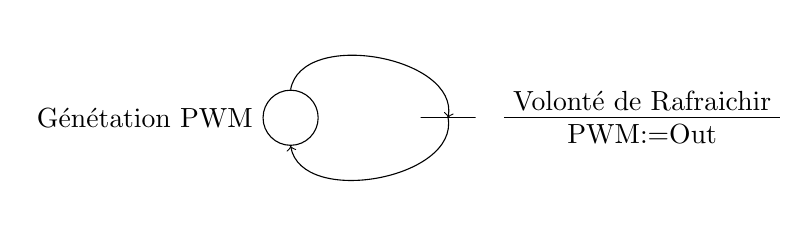
\begin{tikzpicture}

\node[Etape,label=left:Génétation PWM] (I) {};

\node[Trans,node distance = 2cm,align=center,right of=I] (T) {};
\node[Line,align=center,anchor=west,at =(T.east),xshift=10pt] {Volonté de Rafraichir\\PWM:=Out};

\draw[->] (I) edge [bend left=90] (T);
\draw[->] (T) edge [bend left=90] (I);

\end{tikzpicture}




